\clearpage
\begin{flushright}
  \fechaclase{22 de septiembre de 2026}
\end{flushright}

Considere el sistema de segundo orden
\[
  \dot{X}_1=X_2
\]
\[
  \dot{X}_2=f(X,t)+u
\]
\[
  y=X_1
\]

Se desea realizar seguimiento de trayectorias con atenuación de
\textit{chattering} con el error $e=r-y$ y la superficie de deslizamiento
\[
  \sigma=\dot{e}+me+m\int e\,dt
\]

Se deriva el error
\[
  \dot{e}=\dot{r}-\dot{y}=\dot{r}-\dot{X}_1=\dot{r}-X_2
\]
\[
  \ddot{e}=\ddot{r}-\dot{X}_2=\ddot{r}-f(X,t)-u
\]
y la superficie de deslizamiento
\[
  \dot{\sigma}=\ddot{e}+m\dot{e}+me
\]
\[
  \dot{\sigma}=\ddot{r}+m\dot{r}-mX_2-f(X,t)+me-u
\]

Y se propone la función de Lyapunov
\[
  V=\frac{1}{2}\sigma^2
\]
con derivada
\[
  \dot{V}=\sigma\dot{\sigma}
  =\sigma\left[\ddot{r}+m\dot{r}-f(X,t)-mX_2+me\right]-\sigma u
\]
Suponiendo que
\[
  \left\lvert\ddot{r}+m\dot{r}-f(X,t)\right\rvert\leq L
\]
para algún $L$ positivo, se tiene
\[
  \dot{V}\leq L\lvert\sigma\rvert
  +m\lvert X_2\rvert\lvert\sigma\rvert
  +m\lvert e\rvert\lvert\sigma\rvert-\sigma u
\]
Se propone el controlador
\[
  u=K V_{eq}\operatorname{sign}(\sigma)
\]
\[
  V_{eq}=L+m\lvert X_2\rvert+m\lvert e\rvert
\]
Sustituyendo
\[
  \dot{V}\leq
  \left(L+m\lvert X_2\rvert+m\lvert e\rvert\right)
  \lvert\sigma\rvert-KV_{eq}\lvert\sigma\rvert
\]
\[
  \dot{V}\leq V_{eq}\lvert\sigma\rvert
  -KV_{eq}\lvert\sigma\rvert
\]
\[
  \dot{V}\leq-(K-1)V_{eq}\lvert\sigma\rvert
\]
Mostrando que el controlador
\[
  V_{eq}=L+m\lvert X_2\rvert+m\lvert e\rvert
\]
\[
  \sigma=\dot{e}+me+m\int e\,dt
\]
\[
  u=KV_{eq}\operatorname{sign}(\sigma)
\]
estabiliza el sistema.

\paragraph{\tituloejemplo{Ejemplo}}
Verifique el funcionamiento del controlador para
\[
  \dot{X}_1=X_2
\]
\[
  \dot{X}_2=\operatorname{sen}(X_1X_2)+\cos(X_1+X_2)+u
\]
\[
  y=X_1
\]

\paragraph{Resolución}

El controlador se implementa dentro de un bloque \texttt{MATLAB Function}:

\begin{MatlabCode}
function u = controlador(e, de, ie, x1, x2)

% Ganancia K>1
K = 3;

% Valor arbitrario positivo
m1 = 2;
m2 = 2.2;
L = 0.8; % Amplitud máxima de mi sistema

Veq = L + m1*abs(x2)+m2*abs(e);
sigma = de + m1*e + m2*ie;
u = K*Veq*sign(sigma);
\end{MatlabCode}

La planta también se implementa dentro de un bloque
\texttt{MATLAB Function}:

\begin{MatlabCode}
function [dx1, dx2, y] = planta(x1, x2, u)

dx1 = x2;
dx2 = sin(x1+x2) + cos(x1*x2) + u;

y = x1;
\end{MatlabCode}

\begin{center}
  \href{file:../../sim/Parcial\%201/}{%
    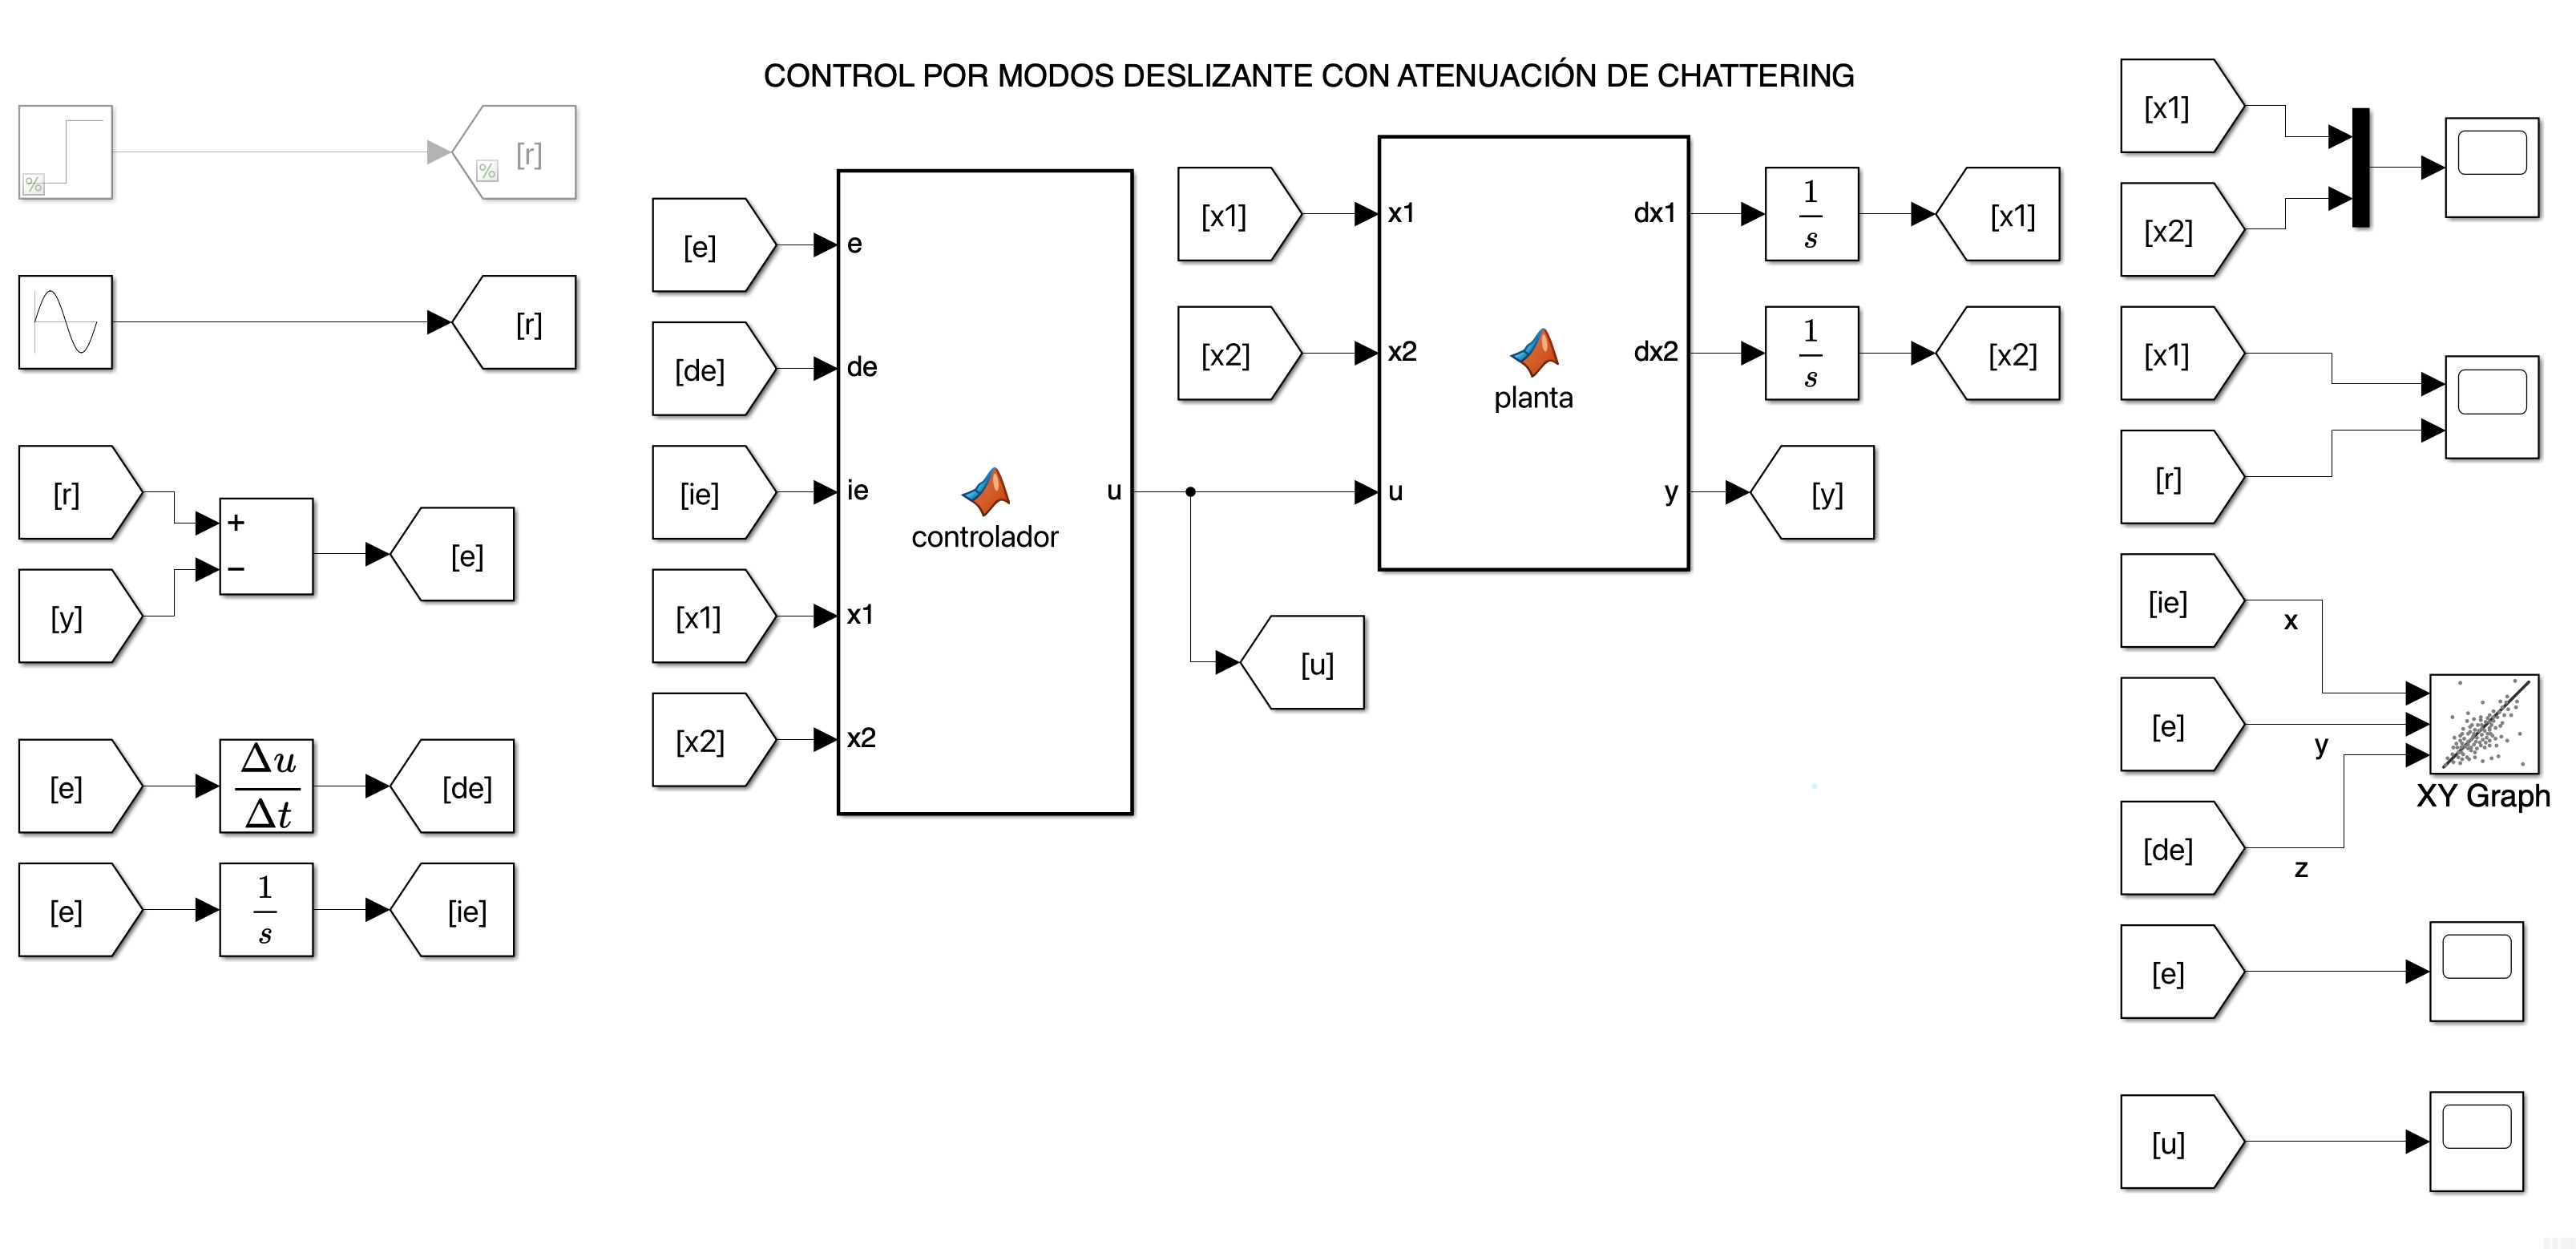
\includegraphics[width=0.85\textwidth]{img/SMC_atenuacionChattering_seg_tray_V2.png}%
  }

  \small\textit{Haga clic en la imagen para abrir la carpeta de los modelos de Simulink y abra el archivo \texttt{EjemploSMC\_seg\_tray\_atenuacion\_chattering\_V2.slx} para ejecutar la simulación.}
\end{center}
